\section{System Overview of \sysname}
\label{sec:System}

%Before that, let's take an overview of the components in \sysname in the pipeline order.
This section overviews the three main components of \sysname, whose workflow is illustrated in Figure~\ref{fig:SystemPipeline}.

\begin{figure*}[htbp]
\centerline{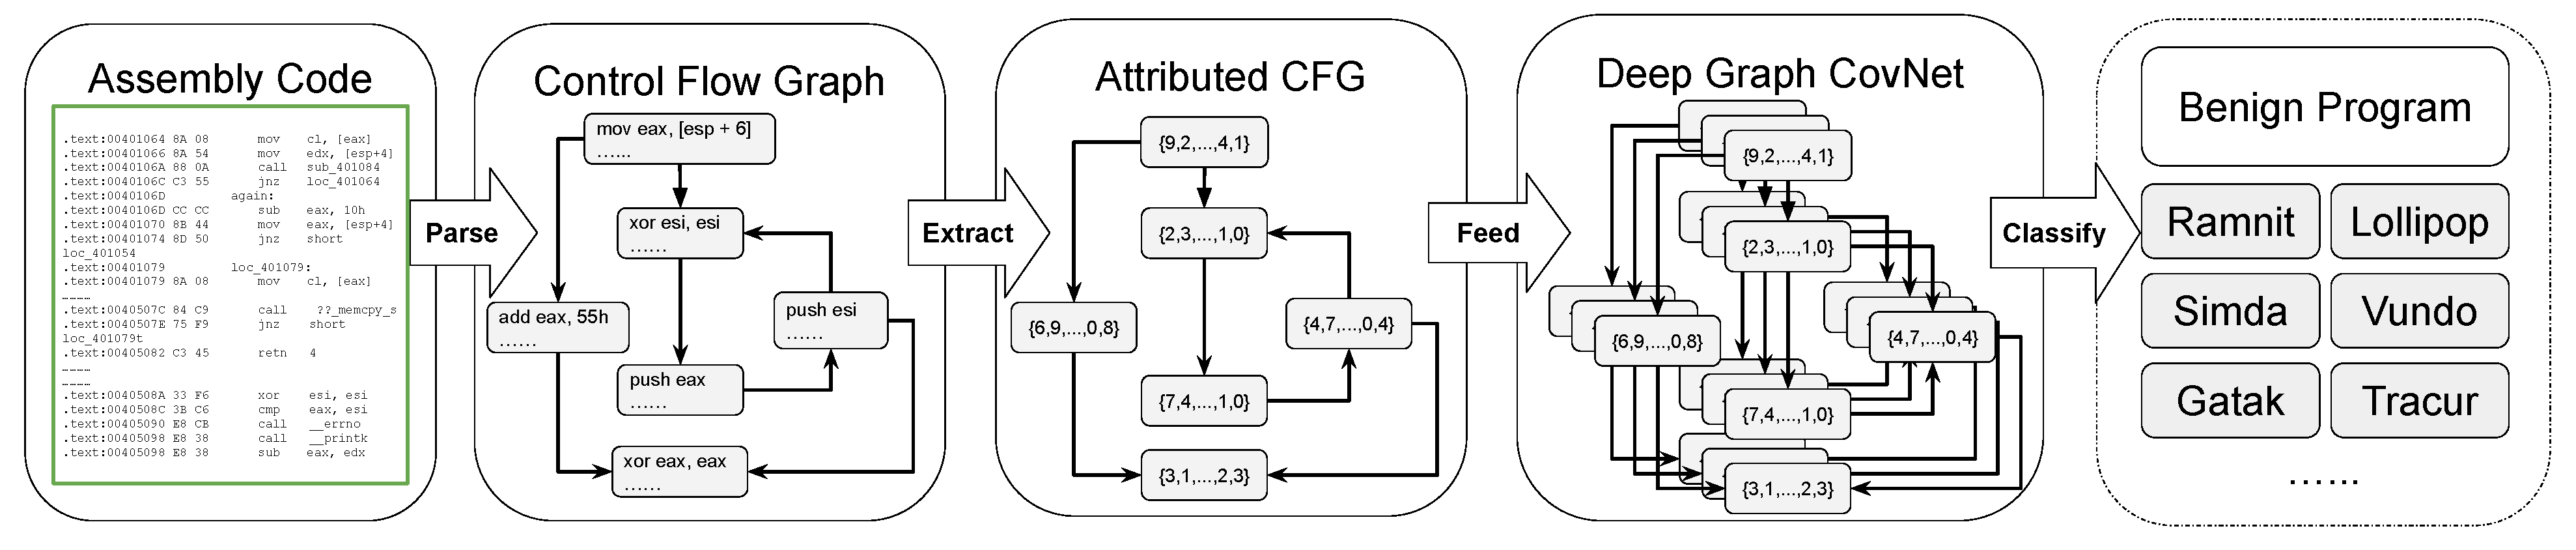
\includegraphics[width=1.0\textwidth]{Magic/figures/SystemPipeline.eps}}
\caption{The workflow of \sysname, a DGCNN-based malware classification system}
\label{fig:SystemPipeline}
\end{figure*}

\subsection{Control Flow Graph}\label{subsec:ConstructCfg}
%Given a cross-platform assembly code, 

\sysname relies on the state-of-the-art tools, such as IDA Pro~\cite{bib:idapro}, to extract CFGs from malware code.
In a CFG, a vertex represents a basic block, which contains a straight sequence of code or assembly instructions without any control flow transition except at its exit.
Two vertices $(u, v)$ are connected by a directed edge $u \rightarrow v$ if either the last instruction in $u$ falls through the first line of code in $v$,
or there is a jump instruction in $u$ that is destined to some instructions (e.g., jump target) in $v$.
The implementation details on how to build the CFG from disassembled execution code will be given in Section~\ref{sec:BuildCfg}.

\subsection{Attributed Control Flow Graph}\label{subsec:Cfg2Acfg}
The CFG representation of software program is generic for the purpose of malware classification in several ways.
First, this type of representation transcends specific programming languages in which the programs are written or hardware platforms for which the programs are developed.
Although other low-level representations such as hexadecimal byte sequences have similar properties, a CFG explicitly expresses the execution logic of a program using a graph data structure.
Hence, the semantics of a malware program is embodied by not only the characteristics of the code in individual basic blocks but also their structural dependencies defined by the edges connecting these basic blocks. 


%which can be used as raw features us works on ML-based malware classification but also 

%The expressive power of CFGs also enables the collection of a variety of aggregate features


%Furthermore, the vertices in the graph provide us a suitable unit environment to extract code-level attributes, many of which are scatteringly adopted by existing machine learning models as raw features.

To convert CFGs to structures that are amenable to machine learning, we define attributes at each vertex that summarize code characteristics as numerical values.
Initially the attributes computed at a vertex do not contain any structural information, which means that their values are independently collected from the corresponding basic block.
Table~\ref{tab:UsedAttributes} lists the attributes implemented in our prototype system, although more attributes can be conveniently added to further improve malware classification performance.

\begin{table}[htbp]
\caption{Block-level attributes used in \sysname}
\begin{center}
\begin{tabular}{c|l}
\hline
Attribute Type & Attribute Description \\
\hline
\multirow{10}{*}{From Code Sequence} & \# Numeric Constants \\
 & \# Transfer Instructions         \\
 & \# Call Instructions             \\
 & \# Arithmetic Instructions       \\
 & \# Compare Instructions          \\
% & \# Crypto instructions           \\
 & \# Mov Instructions              \\
 & \# Termination Instructions      \\
 & \# Data Declaration Instructions \\
 & \# Total Instructions            \\
\hline
\multirow{2}{*}{From Vertex Structure} & \# Offspring, i.e., Degree \\
 & \# Instructions in the Vertex    \\
 \hline
\end{tabular}
\label{tab:UsedAttributes}
\end{center}
\end{table}

As the raw attributes in an attributed CFG (ACFG) contain little structural information and the number of vertices in an ACFG varies with the individual program from which the CFG is derived, for the purpose of malware classification it is necessary to aggregate these attributes over all the vertices in the ACFG in an organic manner depending on its graph structure.
The task of such attribute aggregation is accomplished with DGCNN, which shall be explained next.

%Figure~\ref{fig:SystemPipeline} shows how the further processing on the vertices of a CFG offers us the attributed CFG representation.

%Attributes are numeric values that characterize a vertex in a CFG.
%It usually describes the sequence of code inside a code block, such as the number of constants and the number of transfer instructions.
%It also includes structural information of the vertex, such as the number of offspring and betweenness.


\subsection{Deep Graph Convolution Neural Network}\label{subsec:DGCNN}
Unlike image or text-based data, graph-based data are of variable sizes and are thus not naturally ordered tensors.
%Therefore, a gap exists between the ACFG and the optimal features on the basis of which a machine-learning-powered detection engine makes malware prediction. In our pipeline, this gap is bridged by 
To address this challenge, we use the state-of-the-art deep neural network that can automatically learn discriminative latent features from malware data abstracted as ACFGs.
Particularly, we use deep graph convolution neural network to transform unordered graph data of varying sizes to tensors of fixed size and order.
The transformation algorithm first recursively propagates the weighted attributes in each vertex through the neighborhood defined by the graph structure.
Next, it sorts the vertices in the order of their feature descriptors.
After the sorting step, the graphs with variant sizes are embedded into fixed-size vectors, which are amenable to ML-based classification.
In the next section, we shall elaborate on these operations as well as our extensions based on formal mathematical descriptions.
